\section{Omni XcalableACC Compiler}

We have developed the Omni XACC compiler as the reference implementation
of XACC compilers.
% Omni XACC works internally as a source-to-source compiler that translates XACC programs 
% into those in the base languages with runtime calls.

\begin{figure}[h]
\centering
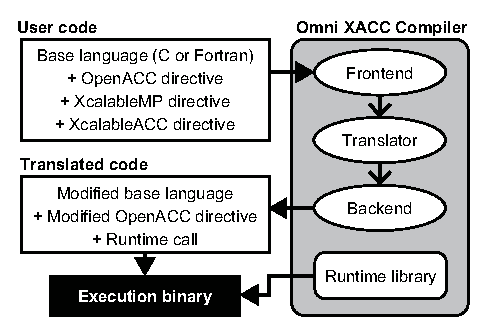
\includegraphics[scale=0.94,clip]{figs/flow2.eps}
\caption{Compile flow of Omni XcalableACC Compiler}
\label{fig:flow}
\end{figure}

Fig.~\ref{fig:flow} shows the compile flow of Omni XACC.
First, 
Omni XACC accepts XACC source codes and translates them into those in
the base languages with runtime calls.
%
Next, the translated code is compiled by a native compiler, which
supports OpenACC, to generate an object file.
%
Finally, the object files and the runtime library are linked by the
native compiler to generate an execution file.
%For details on how Omni Compiler translates the user code, please refer to section V of \cite{nakao2014}.

% \begin{figure}[!t]
% \begin{center}
% \begin{lstlisting}
% double a[N];
% #pragma xmp template t[N]
% #pragma xmp nodes p[4]
% #pragma xmp distribute t[block] onto p
% #pragma xmp align a[i] with t[i]
% ...
% #pragma acc data copy(a)
% {
% #pragma xmp loop on t[i]
% #pragma acc parallel loop
%   for(int i=0;i<N;i++){ 
%     a[i] = ... ;
%   }
% }
% \end{lstlisting}
% \end{center} 
% \caption{Example of XcalableACC code} \label{fig:program}
% \end{figure}

% \begin{figure}[h]
% \begin{center}
% \begin{lstlisting}
% long long _XACC_start_a  = _XACC_get_array_start_index(_XMP_DESC_a, 0);
% long long _XACC_length_a = _XACC_get_array_length(_XMP_DESC_a, 0, N-1);
% #pragma acc data copy(_XMP_ADDR_a[_XACC_start_a:_XACC_length_a])
% {
%   int _XMP_loop_init_i;
%   int _XMP_loop_cond_i;
%   int _XMP_loop_step_i;
%   _XMP_sched_loop_template_BLOCK(0, N, 1, &(_XMP_loop_init_i), &(_XMP_loop_cond_i), &(_XMP_loop_step_i), ...);
% #pragma acc parallel loop
%   for(int i = _XMP_loop_init_i; i < _XMP_loop_cond_i; i += _XMP_loop_step_i) {
%      (*(_XMP_M_GET_ADDR_E_1(_XMP_ADDR_a, i))) = ... ;
%   } // end for
% } // end acc data
% \end{lstlisting}
% \end{center} 
% \caption{Example of loop statement translation using Omni XcalableACC Compiler} \label{fig:program2}
% \end{figure}

% %In order to perform parallelization of a loop statement using both XMP and OpenACC, 
% Omni XACC Compiler dynamically allocates a reasonable memory for distributed arrays.
% According to the OpenACC specification, 
% when using dynamic memory allocation, 
% the start index and length of the array must be specified in the OpenACC data directive.
% Therefore, when using a distributed array in the OpenACC data directive,
% Omni XACC Compiler must insert the start index and length of the array.
% For example, Omni XACC Compiler translates {\bf \#pragma acc data copy(a)} into {\bf \#pragma acc data copy(a[start:length])} if an array {\bf a} is a distributed array.
% The variables {\bf start} and {\bf length} are the start index and length of the distributed array on each node.
% Omni XACC Compiler also inserts functions to calculate these values before the OpenACC data directive.
% For example, lines 7 to 14 of Figure \ref{fig:program} are translated into  Figure \ref{fig:program2}.
% %Omni XACC compiler translates the XMP loop directive and the loop statement.
% %Next, Omni XACC compiler inserts the OpenACC {\bf parallel} directive before the loop statement.
% %These translations are also shown in lines 5 to 12 of Fig. \ref{fig:program2}.
% In line 8 of Fig. \ref{fig:program2}, {\bf \_XMP\_sched\_loop\_template\_BLOCK()} calculates indexes of a loop statement assigned with each node,
% and these indexes are used in conditions of the loop statement.
% Moreover, 
% a distributed array in the loop statement is translated into a pointer calculation.
% For example, {\bf \_XMP\_M\_GET\_ADDR\_E\_1()} in Fig. \ref{fig:program2} is an XMP macro to calculate a local index from a global index.

In particular, for the data transfer between NVIDIA GPUs across
nodes, we have implemented the following three methods in Omni XACC as
follows:

\begin{enumerate}
  \item[(a)] TCA/IB hybrid communication
  \item[(b)] GPUDirect RDMA with CUDA-Aware MPI
  \item[(c)] MPI and CUDA
\end{enumerate}

Item (a) performs communication with the smallest latency, but it
requires a computing environment equipped with the Tightly Copuled
Accelerator (TCA) feature\cite{tca,tca2}.
%
Item (b) is superior in performance to Item (c), but also
requires specific software and hardware (e.g., MVAPICH2-GDR and Mellanox
InfiniBand).
%
Whereas (a) and (b) can realize direct communication between GPUs
without the intervention of CPU, 
%
Item (c) cannot. It copies the data from accelerator memory to 
host memory using CUDA and then transfers the data to other compute
nodes using MPI.
Therefore, although its performacnce is the lowest, it requires neither
specific software nor hardware.
